\chapter{Théorie de Hückel et systèmes conjugués}\label{ch:b2:huckel}

L'hydrogénation du cyclohexène libère \qty{119}{kJ} par mole. Le benzène,
avec trois doubles liaisons dans un cycle de six carbones, devrait en libérer trois fois
plus en devenant cyclohexane~; il en libère \qty{150}{kJ} de moins. Cette énergie
manquante est la stabilité d'un cycle \omterm{def:b2:huckel:aromatic}{aromatique}, la raison pour laquelle le benzène résiste
aux additions que subissent les alcènes. En 1931, Erich Hückel l'a calculée à l'aide d'un
déterminant, après avoir réduit la molécule à ses électrons $\pi$ et à leurs
voisins. Sa méthode est grossière, mais elle explique pourquoi les cycles à six électrons $\pi$
sont particuliers, pourquoi les longues chaînes conjuguées absorbent la lumière visible, et
où une molécule conjuguée porte ses charges.

\begin{recall}
\Cref{ch:b2:diatomic-mos}~: \omterm{def:b2:diatomic-mos:integrals}{intégrale coulombienne} $\alpha$, \omterm{def:b2:diatomic-mos:integrals}{intégrale de résonance} $\beta$,
\omterm{def:b2:diatomic-mos:integrals}{déterminant séculaire}. \Cref{ch:b2:fragment-orbitals}~: orbitales $\pi$ de l'éthène et
de l'allyle. Le volume de première année~: systèmes conjugués, mésomérie, chromophores et
maximums d'absorption.
\end{recall}

\section{La méthode de Hückel}

Dans une molécule conjuguée plane, les orbitales $\sigma$ sont symétriques et les orbitales p
perpendiculaires au plan antisymétriques par rapport à ce plan~: elles
ne se mélangent pas (\cref{prop:b2:diatomic-mos:symmetry}), et l'on peut traiter les
électrons $\pi$ à part.

\begin{definition}[Méthode de Hückel]\label{def:b2:huckel:method}
La \emph{méthode de Hückel}\index{methode de Huckel@méthode de Hückel} calcule les orbitales $\pi$ d'un
système conjugué plan comme combinaisons $\psi = \sum_r c_r p_r$ d'une orbitale p par
atome, avec les approximations suivantes~: recouvrements $S_{rs} = 0$ pour $r \neq s$ (et 1 pour $r =
s$)~; \omterm{def:b2:diatomic-mos:integrals}{intégrales coulombiennes} toutes égales à $\alpha$~; \omterm{def:b2:diatomic-mos:integrals}{intégrales de résonance} égales à $\beta < 0$
entre voisins liés et nulles sinon.
\end{definition}

Avec $x = (\alpha - E)/\beta$, les équations séculaires deviennent, pour chaque atome $r$,
$xc_r + \sum_{s \text{ lié à } r} c_s = 0$, et les énergies sont les racines d'un
déterminant portant $x$ sur la diagonale et 1 entre atomes liés. De façon équivalente, $E =
\alpha + m\beta$, où les $m$ sont les valeurs propres de la matrice d'adjacence du
squelette carboné de la molécule~; comme $\beta < 0$, un $m$ positif correspond à un niveau liant.

\begin{method}[Un calcul de Hückel]\label{met:b2:huckel:huckel}
\begin{enumerate}
  \item Numéroter les atomes conjugués~; écrire la matrice avec 0 sur la diagonale et 1
        pour chaque paire liée.
  \item Trouver ses valeurs propres $m_k$ (par les formules explicites ci-dessous, ou numériquement)~: $E_k =
        \alpha + m_k\beta$.
  \item Remplir les niveaux à partir du plus liant, deux électrons chacun~:
        $E_\pi = \sum_k n_k E_k$.
  \item À partir des coefficients normalisés, calculer les charges et les indices de liaison.
\end{enumerate}
\end{method}

\begin{proposition}[Trace]\label{prop:b2:huckel:trace}
Les énergies des $n$ orbitales $\pi$ d'un système de Hückel ont pour somme $n\alpha$.
\end{proposition}

\begin{proof}
La somme des valeurs propres d'une matrice est sa trace~; la matrice de Hückel porte $\alpha$
sur chacun de ses $n$ termes diagonaux.
\end{proof}

\section{Les polyènes linéaires}

\begin{theorem}[Niveaux d'une chaîne linéaire]\label{thm:b2:huckel:polyene}
Une chaîne conjuguée linéaire de $n$ atomes a pour niveaux et coefficients
\[
  E_k = \alpha + 2\beta\cos\frac{k\pi}{n + 1}, \qquad
  c_{jk} = \sqrt{\frac{2}{n + 1}}\,\sin\frac{jk\pi}{n + 1}, \qquad k = 1, \dots, n .
\]
\end{theorem}

\begin{proof}
Les équations séculaires sont $c_{j-1} + xc_j + c_{j+1} = 0$ pour $j = 1, \dots, n$, avec
$c_0 = c_{n+1} = 0$. Essayons $c_j = \sin j\theta$~: $\sin(j - 1)\theta + \sin(j + 1)\theta = 2\sin
j\theta\cos\theta$, de sorte que les équations sont vérifiées avec $x = -2\cos\theta$, et $c_0 = 0$
automatiquement. La condition au bout $c_{n+1} = \sin(n + 1)\theta = 0$ donne $\theta =
k\pi/(n + 1)$. Alors $E = \alpha - x\beta = \alpha + 2\beta\cos\theta$. La normalisation utilise
$\sum_{j=1}^n\sin^2 j\theta = (n + 1)/2$.
\end{proof}

\begin{example}[Le butadiène]\label{ex:b2:huckel:butadiene}
Pour $n = 4$~: $E = \alpha \pm 1.618\beta$, $\alpha \pm 0.618\beta$. Quatre électrons $\pi$ remplissent les deux
niveaux liants~: $E_\pi = 4\alpha + 2(1.618 + 0.618)\beta = 4\alpha + 4.472\beta$. L'orbitale la plus basse
a pour coefficients 0.372, 0.602, 0.602, 0.372, la suivante 0.602, 0.372,
$-0.372$, $-0.602$.
\end{example}

\begin{omfigure}
\begin{tikzpicture}[font=\small]
  \foreach \k/\a/\b/\c/\d/\lab in {1/0.372/0.602/0.602/0.372/{$\psi_1$, $\alpha + 1.618\beta$},
      2/0.602/0.372/-0.372/-0.602/{$\psi_2$, $\alpha + 0.618\beta$},
      3/0.602/-0.372/-0.372/0.602/{$\psi_3$, $\alpha - 0.618\beta$},
      4/0.372/-0.602/0.602/-0.372/{$\psi_4$, $\alpha - 1.618\beta$}} {
    \begin{scope}[yshift={(\k-1)*2.1cm}]
      \draw[black!40] (-0.2,0) -- (3.2,0);
      \pic at (0,0) {omp={1.6*\a}{90}}; \pic at (1,0) {omp={1.6*\b}{90}};
      \pic at (2,0) {omp={1.6*\c}{90}}; \pic at (3,0) {omp={1.6*\d}{90}};
      \node[anchor=west] at (3.6,0) {\lab};
    \end{scope}
  }
\end{tikzpicture}

{\small Les quatre orbitales $\pi$ du butadiène, lobes dessinés proportionnellement aux
coefficients de Hückel (calculés) et colorés selon leur signe~; les énergies croissent
vers le haut, avec $0, 1, 2, 3$ nœuds. Les deux orbitales inférieures sont remplies.}
\end{omfigure}

\begin{definition}[Charges $\pi$ et indices de liaison]\label{def:b2:huckel:indices}
Avec $n_k$ électrons dans l'orbitale $k$ (0, 1 ou 2) et des coefficients réels $c_{rk}$, la
\emph{charge $\pi$}\index{charge pi@charge $\pi$} de l'atome $r$ est $q_r = \sum_k n_kc_{rk}^2$ (le
nombre d'électrons $\pi$ qu'il porte), et l'\emph{indice de liaison $\pi$}\index{indice de liaison pi@indice de liaison $\pi$}
de la liaison $rs$ est $p_{rs} = \sum_k n_kc_{rk}c_{sk}$.
\end{definition}

Pour le butadiène, $p_{12} = 2(0.372 \times 0.602 + 0.602 \times 0.372) = 0.894$ et $p_{23} =
2(0.602^2 - 0.372^2) = 0.447$~: les liaisons terminales portent l'essentiel de la liaison $\pi$ et sont
les plus courtes, la liaison centrale a un caractère partiel de double liaison. Toutes les charges valent
1.

\begin{proposition}[Hydrocarbures alternants]\label{prop:b2:huckel:alternant}
Dans un hydrocarbure neutre dont les atomes conjugués peuvent être répartis en deux ensembles sans
que deux voisins appartiennent au même ensemble (pas de cycle impair), toutes les charges $\pi$ valent 1.
\end{proposition}

\admitted

Ce résultat (Coulson et Rushbrooke) se vérifie ci-dessus sur le butadiène et sur le benzène par
symétrie~; c'est la raison pour laquelle de tels hydrocarbures n'ont pas de moment dipolaire permanent dû à leurs
électrons $\pi$.

\begin{definition}[Énergie de délocalisation]\label{def:b2:huckel:delocalisation}
L'\emph{énergie de délocalisation}\index{energie de delocalisation@énergie de délocalisation} d'un système
conjugué est la différence entre son énergie $\pi$ et celle du même nombre de
doubles liaisons isolées, chacune d'énergie $E_\pi = 2\alpha + 2\beta$.
\end{definition}

Pour le butadiène, elle vaut $4.472\beta - 4\beta = 0.472\beta$~; pour l'hexatriène, $0.988\beta$.

\section{Cycles et aromaticité}

\begin{theorem}[Niveaux d'un cycle]\label{thm:b2:huckel:ring}
Un cycle plan de $n$ atomes conjugués a pour niveaux $E_k = \alpha + 2\beta\cos(2\pi k/n)$,
$k = 0, 1, \dots, n - 1$~: un niveau le plus bas $\alpha + 2\beta$, puis des paires de niveaux
dégénérés et, pour $n$ pair, un niveau le plus haut $\alpha - 2\beta$.
\end{theorem}

\begin{proof}
Dans un cycle, chaque atome a deux voisins, les indices étant pris modulo $n$~:
$c_{j-1} + xc_j + c_{j+1} = 0$ pour tout $j$ et $c_{j+n} = c_j$. Essayons $c_j = \mathrm e^{\mathrm
i jq}$~: l'équation donne $x = -(\mathrm e^{-\mathrm iq} + \mathrm e^{\mathrm iq}) = -2\cos q$,
et la périodicité exige $nq = 2\pi k$. Les niveaux $k$ et $n - k$ ont la même
énergie~; leur somme et leur différence sont des orbitales réelles. Seul $k = 0$ (et $k = n/2$ pour
$n$ pair) est simple.
\end{proof}

\begin{corollary}[Cercle de Frost]\label{cor:b2:huckel:frost}
Les niveaux d'un cycle se lisent sur un cercle de rayon $2|\beta|$ centré en $\alpha$, dans
lequel on inscrit un $n$-gone régulier avec un sommet en bas~: chaque sommet est
à la hauteur d'un niveau.
\end{corollary}

\begin{proof}
Le sommet $k$ du polygone se trouve à l'angle $-\pi/2 + 2\pi k/n$, et donc à la hauteur
$-2|\beta|\cos(2\pi k/n) = 2\beta\cos(2\pi k/n)$ par rapport au centre.
\end{proof}

\begin{omfigure}
\begin{tikzpicture}[font=\scriptsize]
  \foreach \n/\x/\name/\el in {4/0/{\ce{C4H4}}/4, 5/3.4/{\ce{C5H5-}}/6, 6/6.8/{\ce{C6H6}}/6, 7/10.2/{\ce{C7H7+}}/6} {
    \begin{scope}[xshift=\x cm]
      \draw[black!35] (0,0) circle (1.2);
      \draw[black!60] \foreach \k in {0,...,\the\numexpr\n-1\relax} { ({-90+360*\k/\n}:1.2) -- ({-90+360*(\k+1)/\n}:1.2) };
      \foreach \k in {0,...,\the\numexpr\n-1\relax} {
        \draw[very thick] ({1.2*cos(-90+360*\k/\n)-0.22},{1.2*sin(-90+360*\k/\n)}) -- ({1.2*cos(-90+360*\k/\n)+0.22},{1.2*sin(-90+360*\k/\n)});
      }
      \draw[densely dotted] (-1.5,0) -- (1.5,0);
      \node[font=\small] at (0,-1.75) {\name};
    \end{scope}
  }
  \node[anchor=east] at (-1.5,0) {$\alpha$};
  % electrons: C4H4 (2 + 1 + 1), others filled lowest three
  \foreach \x in {0,3.4,6.8,10.2} {
    \draw[-{Stealth[length=1mm]}, thick] ({\x-0.05},-1.32) -- ({\x-0.05},-1.08);
    \draw[-{Stealth[length=1mm]}, thick] ({\x+0.05},-1.08) -- ({\x+0.05},-1.32);
  }
  % six-electron rings: the lowest degenerate pair is filled
  \foreach \n/\x in {5/3.4, 6/6.8, 7/10.2} {
    \foreach \k in {1, \the\numexpr\n-1\relax} {
      \pgfmathsetmacro\ex{\x + 1.2*cos(-90 + 360*\k/\n)}
      \pgfmathsetmacro\ey{1.2*sin(-90 + 360*\k/\n)}
      \draw[-{Stealth[length=1mm]}, thick] ({\ex-0.05},{\ey-0.12}) -- ({\ex-0.05},{\ey+0.12});
      \draw[-{Stealth[length=1mm]}, thick] ({\ex+0.05},{\ey+0.12}) -- ({\ex+0.05},{\ey-0.12});
    }
  }
  % C4H4: one electron in each of the two nonbonding levels
  \draw[-{Stealth[length=1mm]}, thick] (1.2,-0.12) -- (1.2,0.12);
  \draw[-{Stealth[length=1mm]}, thick] (-1.2,-0.12) -- (-1.2,0.12);
\end{tikzpicture}

{\small Cercles de Frost. Les sommets de chaque polygone, inscrit avec un sommet en
bas dans un cercle de rayon $2|\beta|$, donnent les niveaux du cycle. Avec six électrons $\pi$,
\ce{C5H5-}, \ce{C6H6} et \ce{C7H7+} remplissent le niveau le plus bas et une paire
dégénérée~: couches complètes. Les quatre électrons du cyclobutadiène laissent deux électrons dans une
paire non liante dégénérée (représentée).}
\end{omfigure}

\begin{definition}[Aromaticité]\label{def:b2:huckel:aromatic}
Un système cyclique, plan et entièrement conjugué est \emph{aromatique}\index{aromatique} lorsque
ses électrons $\pi$ forment une couche complète avec une grande \omterm{def:b2:huckel:delocalisation}{énergie de délocalisation}, et
\emph{antiaromatique}\index{antiaromatique} lorsque ses électrons $\pi$ remplissent à moitié une paire
dégénérée, ce qui le rend moins stable que la chaîne ouverte correspondante.
\end{definition}

\begin{theorem}[Règle de Hückel]\label{thm:b2:huckel:huckel-rule}
Un système conjugué monocyclique plan possède une couche complète d'électrons $\pi$ si et seulement
s'il en contient $4N + 2$ ($N = 0, 1, 2, \dots$)~; avec $4N$, il a deux électrons dans une
paire dégénérée à moitié remplie. C'est la \emph{règle de Hückel}\index{regle de Huckel@règle de Hückel}.
\end{theorem}

\begin{proof}
D'après le \cref{thm:b2:huckel:ring}, les niveaux à partir du bas sont un niveau simple puis
des paires dégénérées (pour la partie occupée). Une couche complète remplit le niveau
simple (2 électrons) et un nombre entier $N$ de paires (4 électrons chacune)~: $4N + 2$. Avec
$4N$ électrons, la dernière paire n'en contient que deux, un dans chacune de ses orbitales (règle de
Hund).
\end{proof}

\begin{method}[Est-il aromatique~?]\label{met:b2:huckel:aromaticity}
\begin{enumerate}
  \item Le système est-il un cycle portant une orbitale p sur chaque atome (en comptant les centres
        carbocationiques et carbanioniques et les doublets non liants des hétéroatomes)~?
  \item Peut-il être plan~?
  \item Compter les électrons $\pi$~: $4N + 2$, \omterm{def:b2:huckel:aromatic}{aromatique}~; $4N$, \omterm{def:b2:huckel:aromatic}{antiaromatique} s'il est plan.
  \item Un cycle \omterm{def:b2:huckel:aromatic}{antiaromatique} évite la planéité ou la conjugaison quand il le peut
        (le cyclooctatétraène a la forme d'une baignoire et se comporte comme un polyène).
\end{enumerate}
\end{method}

\begin{example}[Le benzène]\label{ex:b2:huckel:benzene}
Six électrons $\pi$ remplissent $\alpha + 2\beta$ et la paire $\alpha + \beta$~: $E_\pi = 6\alpha + 8\beta$.
Trois doubles liaisons isolées donnent $6\alpha + 6\beta$~: l'\omterm{def:b2:huckel:delocalisation}{énergie de délocalisation} vaut $2\beta$,
environ deux fois celle de la chaîne ouverte à six carbones, l'hexatriène ($0.988\beta$)~: fermer
le cycle en apporte autant de nouveau. Par symétrie, tous les indices de liaison sont égaux ($p = 2/3$), de même que les six
longueurs de liaison, \qty{139.7}{pm}, comprises entre celles de l'éthène (\qty{133.9}{pm}) et de l'éthane
(\qty{153.6}{pm}).
% ledger: geo:C6H6.rCC, geo:C2H4.rCC, geo:C2H6.rCC
\end{example}

\begin{omfigure}
\begin{tikzpicture}[font=\small, y=0.013cm, x=1.0cm]
  \draw[thick] (0,0) -- (10.5,0);
  \node[anchor=north] at (5.2,-8) {cyclohexane (référence, $\Delta_r H = 0$)};
  % cyclohexene
  \draw[thick, omDef] (0.6,118.8) -- (1.6,118.8); \draw[->, omDef] (1.1,118.8) -- (1.1,4);
  \node[font=\scriptsize, anchor=south, align=center] at (1.1,120) {cyclohexène\\ \qty{118.8}{kJ/mol}};
  % diene
  \draw[thick, omDef] (3.6,227.7) -- (4.6,227.7); \draw[->, omDef] (4.1,227.7) -- (4.1,4);
  \draw[thick, black!45, densely dashed] (4.7,237.6) -- (5.6,237.6);
  \node[font=\scriptsize, anchor=south, black!60] at (5.15,240) {$2 \times 118.8$};
  \node[font=\scriptsize, anchor=east, align=right] at (3.5,227.7) {cyclohexa-1,3-diène\\ \qty{227.7}{kJ/mol}};
  % benzene
  \draw[thick, omDef] (7.6,206.0) -- (8.6,206.0); \draw[->, omDef] (8.1,206.0) -- (8.1,4);
  \node[font=\scriptsize, anchor=east, align=right] at (7.5,206.0) {benzène\\ \qty{206.0}{kJ/mol}};
  \draw[thick, black!45, densely dashed] (7.6,356.4) -- (8.6,356.4);
  \node[font=\scriptsize, anchor=south, black!60] at (8.1,358) {$3 \times 118.8 = 356.4$};
  \draw[<->, omThm, thick] (8.9,206) -- (8.9,356.4) node[midway, right, font=\scriptsize] {\qty{150}{kJ/mol}};
\end{tikzpicture}

{\small Enthalpies d'hydrogénation en cyclohexane en phase gazeuse, d'après les enthalpies
de formation tabulées (barres, hauteur = chaleur libérée). Deux doubles liaisons conjuguées
libèrent \qty{10}{kJ/mol} de moins que deux fois une seule~; le benzène libère \qty{150}{kJ/mol} de moins que
trois fois une seule~: c'est sa stabilisation \omterm{def:b2:huckel:aromatic}{aromatique}.}
% ledger: dfh:C6H6_g, dfh:C6H10_g, dfh:C6H12_g, dfh:C6H8_g
\end{omfigure}

\begin{history}[Le cycle de Kekulé]
\begin{minipage}[t]{0.22\linewidth}
\vspace{0pt}
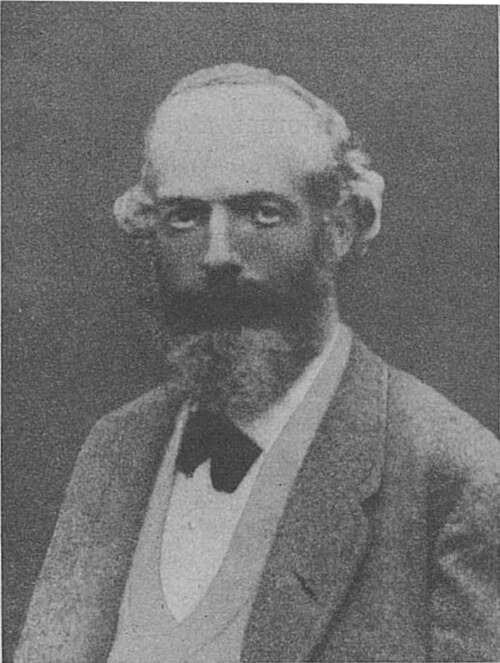
\includegraphics[width=\linewidth]{images/book3/kekule.jpg}
\end{minipage}\hfill
\begin{minipage}[t]{0.74\linewidth}
\vspace{0pt}
En 1865, August Kekulé proposa que les six atomes de carbone du benzène forment un cycle
à liaisons simples et doubles alternées, et peu après que les deux alternances
s'échangent si vite que toutes les liaisons sont identiques. Les liaisons égales mises en évidence par la diffraction
des rayons X, et les orbitales $\pi$ étendues à tout le cycle, donnèrent à son intuition sa
forme moderne~; la \omterm{thm:b2:huckel:huckel-rule}{règle de Hückel}, en 1931, expliqua pourquoi six électrons, et non quatre ou
huit, rendent un cycle particulier. (Portrait, 1873, auteur inconnu, domaine public,
Wikimedia Commons.)
\end{minipage}
\end{history}

\section{Conjugaison et lumière}

\begin{proposition}[L'écart d'un polyène]\label{prop:b2:huckel:gap}
Dans un polyène linéaire de $n$ carbones ($n$ pair), l'écart entre le plus haut niveau occupé
et le plus bas niveau vacant du système $\pi$ vaut $4|\beta|\sin(\pi/(2(n + 1)))$~: il diminue à mesure que la
chaîne s'allonge.
\end{proposition}

\begin{proof}
Le plus haut niveau occupé est $k = n/2$, le plus bas niveau vacant $k = n/2 + 1$. Avec $\theta_k =
k\pi/(n + 1)$, $E_{n/2+1} - E_{n/2} = 2|\beta|(\cos\theta_{n/2} - \cos\theta_{n/2+1}) = 4|\beta|
\sin\frac{\theta_{n/2} + \theta_{n/2+1}}{2}\sin\frac{\theta_{n/2+1} - \theta_{n/2}}{2}$, et le
premier sinus vaut $\sin(\pi/2) = 1$. L'écart diminue quand $n$ augmente puisque $\sin$ est croissant sur
$[0, \pi/2]$.
\end{proof}

\begin{omfigure}
\begin{tikzpicture}
\begin{axis}[width=0.5\linewidth, height=5cm, xmin=0, xmax=22, ymin=0, ymax=2.2,
  axis x line=bottom, axis y line=left, xlabel={nombre de carbones $n$}, ylabel={écart$/|\beta|$},
  tick label style={font=\small}, label style={font=\small}]
\addplot[omThm, thick, mark=*, mark size=1.3pt] table[x=n, y=gap] {figdata/out/bachelor-2-huckel-b.dat};
\end{axis}
\end{tikzpicture}\hfill
\begin{tikzpicture}
\begin{axis}[width=0.48\linewidth, height=5.4cm, xmin=-1, xmax=11, ymin=-2.4, ymax=2.4,
  axis x line=none, axis y line=left, ylabel={$(E - \alpha)/|\beta|$}, clip=false,
  tick label style={font=\small}, label style={font=\small}]
\addplot[only marks, mark=-, mark size=5pt, very thick, omDef] table[x=x, y=e] {figdata/out/bachelor-2-huckel-a.dat};
\draw[densely dotted] (axis cs:-1,0) -- (axis cs:11,0);
\node[anchor=north, font=\scriptsize] at (axis cs:0,-2.45) {C$_2$};
\node[anchor=north, font=\scriptsize] at (axis cs:2,-2.45) {C$_3$};
\node[anchor=north, font=\scriptsize] at (axis cs:4,-2.45) {C$_4$};
\node[anchor=north, font=\scriptsize] at (axis cs:6,-2.45) {C$_6$};
\node[anchor=north, font=\scriptsize] at (axis cs:8,-2.45) {cycle 4};
\node[anchor=north, font=\scriptsize] at (axis cs:10,-2.45) {cycle 6};
\end{axis}
\end{tikzpicture}

{\small À gauche~: l'écart de Hückel des polyènes linéaires diminue quand la chaîne s'allonge,
ce qui explique pourquoi les longues chaînes conjuguées absorbent à de plus grandes longueurs d'onde, jusque dans le visible.
À droite~: niveaux calculés de l'éthène, de l'allyle, du butadiène, de l'hexatriène (chaînes) et du
cyclobutadiène et du benzène (cycles)~; les niveaux liants sont au-dessous de $\alpha$.}
\end{omfigure}

On introduit un hétéroatome en modifiant son \omterm{def:b2:diatomic-mos:integrals}{intégrale coulombienne}, $\alpha_X = \alpha + h\beta$, et les
\omterm{def:b2:diatomic-mos:integrals}{intégrales de résonance} de ses liaisons~: c'est un modèle à paramètres ajustables, qui conserve les
résultats qualitatifs (un atome électronégatif, $h > 0$, attire vers lui la densité $\pi$)
mais dont les nombres sont ajustés, non démontrés.

\section{Exercices}

\begin{exercise}[$\star$]\label{exo:b2:huckel:1}
Donner $E_\pi$ pour le cation, le radical et l'anion allyle.
\end{exercise}

\begin{exercise}[$\star$]\label{exo:b2:huckel:2}
Calculer l'$E_\pi$ du butadiène à partir des niveaux $\alpha \pm 1.618\beta$, $\alpha \pm 0.618\beta$.
\end{exercise}

\begin{exercise}[$\star$]\label{exo:b2:huckel:3}
\omterm{def:b2:huckel:aromatic}{Aromatique}, \omterm{def:b2:huckel:aromatic}{antiaromatique} ou ni l'un ni l'autre (s'il est plan)~: benzène, anion cyclopentadiényle,
cation cyclopentadiényle, cation tropylium \ce{C7H7+}, cyclobutadiène, cyclooctatétraène
plan.
\end{exercise}

\begin{exercise}[$\star$]\label{exo:b2:huckel:4}
Tracer le cercle de Frost du cyclooctatétraène plan et y placer ses huit électrons $\pi$.
\end{exercise}

\begin{exercise}[$\star\star$]\label{exo:b2:huckel:5}
Calculer l'\omterm{def:b2:huckel:delocalisation}{énergie de délocalisation} du butadiène et la donner en \unit{kJ/mol} avec
$|\beta| = \qty{75}{kJ/mol}$. Comparer aux \qty{10}{kJ/mol} tirés des données d'hydrogénation
du cyclohexa-1,3-diène.
\end{exercise}

\begin{exercise}[$\star\star$]\label{exo:b2:huckel:6}
Calculer les indices de liaison $\pi$ du butadiène et prévoir laquelle de ses liaisons C--C est la
plus courte.
\end{exercise}

\begin{exercise}[$\star\star$]\label{exo:b2:huckel:7}
Les niveaux d'un cycle à cinq atomes sont $\alpha + 2\beta$, $\alpha + 0.618\beta$ (deux fois),
$\alpha - 1.618\beta$ (deux fois). Les remplir pour l'anion et le cation cyclopentadiényle et
comparer.
\end{exercise}

\begin{exercise}[$\star\star$]\label{exo:b2:huckel:8}
À l'aide des niveaux d'un cycle à sept atomes, expliquer pourquoi le bromure de cycloheptatriényle
se comporte comme un sel, le bromure de tropylium.
\end{exercise}

\begin{exercise}[$\star\star$]\label{exo:b2:huckel:9}
Vérifier la règle de la trace sur l'hexatriène, dont les niveaux sont $\alpha \pm 1.802\beta$, $\alpha \pm
1.247\beta$, $\alpha \pm 0.445\beta$.
\end{exercise}

\begin{exercise}[$\star\star\star$]\label{exo:b2:huckel:10}
Établir les niveaux de l'hexatriène à partir de la formule explicite, ainsi que son \omterm{def:b2:huckel:delocalisation}{énergie de délocalisation}.
\end{exercise}

\begin{exercise}[$\star\star\star$]\label{exo:b2:huckel:11}
Le cyclobutadiène carré aurait deux électrons célibataires. Expliquer pourquoi la molécule réelle
est rectangulaire, avec deux liaisons courtes et deux longues.
\end{exercise}

\begin{exercise}[$\star\star\star$]\label{exo:b2:huckel:12}
Dans un système $\pi$ à deux atomes \ce{C=X} avec $\alpha_X = \alpha + \beta$ (valeur de modèle, $h = 1$) et
$\beta_{\ce{CX}} = \beta$, trouver les deux niveaux et les charges $\pi$ de C et de X pour deux
électrons.
\end{exercise}

\section{Problème~: l'énergie manquante du benzène}

\begin{problem}[{Problème du week-end --- la stabilisation aromatique du benzène d'après
les enthalpies d'hydrogénation, les niveaux de Hückel du benzène et son énergie de
délocalisation, la valeur de $|\beta|$, et la comparaison avec l'hexatriène et le
cyclooctatétraène}]
\label{pb:b2:huckel:1}
Données~: enthalpies de formation des gaz (\unit{kJ/mol})~: benzène 82.9,
cyclohexa-1,3-diène 104.6, cyclohexène $-4.3$, cyclohexane $-123.1$. Longueurs de liaison
(pm)~: benzène 139.7, éthène 133.9, éthane 153.6.
% ledger: dfh:C6H6_g, dfh:C6H8_g, dfh:C6H10_g, dfh:C6H12_g, geo:C6H6.rCC, geo:C2H4.rCC, geo:C2H6.rCC

\medskip
\noindent\textbf{Partie I --- L'hydrogénation.}
\begin{enumerate}
  \item Calculer le $\Delta_r H^\circ$ de l'hydrogénation du cyclohexène en cyclohexane.
  \item Même question pour le cyclohexa-1,3-diène.
  \item Même question pour le benzène.
  \item Que libéreraient trois doubles liaisons indépendantes~?
  \item En déduire la stabilisation du benzène.
  \item Comparer à celle du diène conjugué, et commenter.
\end{enumerate}

\medskip
\noindent\textbf{Partie II --- Le benzène selon Hückel.}
\begin{enumerate}[resume]
  \item Écrire la matrice de Hückel du benzène.
  \item Donner ses niveaux d'après la formule des cycles.
  \item Les remplir avec six électrons $\pi$.
  \item Calculer $E_\pi$.
  \item Calculer l'$E_\pi$ de trois doubles liaisons isolées.
  \item En déduire l'\omterm{def:b2:huckel:delocalisation}{énergie de délocalisation}.
  \item Vérifier la règle de la trace.
\end{enumerate}

\medskip
\noindent\textbf{Partie III --- La valeur de $|\beta|$.}
\begin{enumerate}[resume]
  \item Égaler l'\omterm{def:b2:huckel:delocalisation}{énergie de délocalisation} à la stabilisation de la partie I et en déduire
        $|\beta|$.
  \item Avec cette valeur, prévoir l'\omterm{def:b2:huckel:delocalisation}{énergie de délocalisation} du butadiène, et la comparer
        à la partie I.
  \item Calculer les indices de liaison $\pi$ du benzène.
  \item Les comparer à ceux du butadiène.
  \item Expliquer pourquoi les longueurs de liaison du benzène sont égales et où elles se situent.
\end{enumerate}

\medskip
\noindent\textbf{Partie IV --- Autres cycles et autres chaînes.}
\begin{enumerate}[resume]
  \item Calculer l'\omterm{def:b2:huckel:delocalisation}{énergie de délocalisation} de l'hexatriène et comparer au benzène.
  \item Donner les niveaux du cyclooctatétraène plan.
  \item Les remplir avec huit électrons~: qu'est-ce qui ne va pas~?
  \item Comment la molécule réelle s'en tire-t-elle~?
  \item Quelle est la situation du cyclobutadiène~?
  \item Énoncer la \omterm{thm:b2:huckel:huckel-rule}{règle de Hückel}.
  \item Donner la valeur de $|\beta|$ obtenue en égalant l'\omterm{def:b2:huckel:delocalisation}{énergie de délocalisation} du benzène
        à sa stabilisation mesurée.
\end{enumerate}
\end{problem}
